\section{Optimizing SGEMM}
\label{sec:optimization}


The demystified GPU microarchitecture features provide us a larger tuning space for computational kernels.
We apply
a series of incremental optimizations to improve SGEMM performance on Kepler architecture. The optimization strategies
go through architectural hierarchy from CUDA core and register to memory. All the optimization strategies are inspired by the observations from our benchmarking.
\begin{itemize}
\item At core level, we orchestrate {\tt FFMA} instruction executions with a more efficient instruction scheduling set by the proper control code.
% with respect to the proper control code pattern.
\item At register level, we meticulously map operands to registers so that bank conflicts are avoided for the inner loop in Algorithm~\ref{gemm}.
\item At memory level, we select appropriate shared memory load/store width and global memory data path to mitigate
latencies.
\end{itemize}
\subsection{Register Allocation}
\label{sec:register}
\begin{figure}[htbp]
\begin{center}
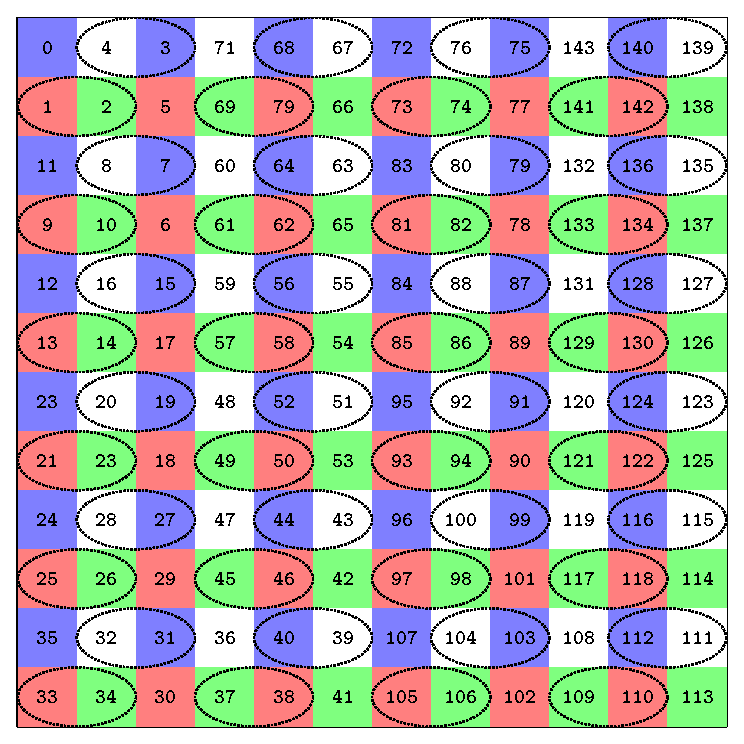
\includegraphics[scale=0.5]{reg}
\caption{Register allocation in SGEMM. The number in the cell is a register index.
Different colors denote the mapping of register banks: green$\rightarrow$bank0,
    blue$\rightarrow$bank1, gray$\rightarrow$bank2, red$\rightarrow$bank3.}
\label{fig:reg}
\end{center}
\end{figure}

To allocate registers for $A$ column, $B$ row, and $C$ sub-matrix as in Algorithm~\ref{gemm}, we have three objectives:
correctness, no bank conflict, and tight register indices.
{\tt LDG.128} restricts four words alignment for registers.
Since NVIDIA GPU does not have $128$-bit registers, 
four consecutive $32$-bit registers {\tt RN}, {\tt RN+1}, {\tt RN+2}, and {\tt RN+3} will be an equivalence for a 128-bit
register.
%a $128$-bit load instruction ({\tt LDG.128}) writes the data to four consecutive $32$-bit registers {\tt RN}, {\tt RN+1}, {\tt RN+2}, and {\tt RN+3} given one destination register $RN$.
% in order to use $128$-bit load, one destination register $RN$ is given,
% results will be written to
% four $32$-bit registers: {\tt RN}, {\tt RN+1}, {\tt RN+2}, {\tt RN+3}.
We discover an undocumented restriction that $N\%4=0$, otherwise illegal instruction errors will be reported.
% It's not hard to understand this restriction,
The four words alignment restriction for {\tt LDG.128} simplifies hardware logic and cuts down power.
Since we use {\tt LDG.128} to load $A$ and $B$, there are two bank allocation choices limited by $N\mod4==0$ restriction and Kepler's bank distribution (Table~\ref{tab:reg}).
We assume allocate bank of $A$ matrix $\begin{bmatrix} 0 \\ 1  \end{bmatrix}$,
   bank of $B$ $\begin{bmatrix} 2 & 3 \end{bmatrix}$ as shown in Figure~\ref{fig:reg}, two choices left for $C$,
$\begin{bmatrix} 1 & 2 \\ 3 & 0  \end{bmatrix}$ and
$\begin{bmatrix} 3 & 1 \\ 0 & 2  \end{bmatrix}$.
The $2\times2=4$ bank patterns for SGEMM are equivalent in performance, then we arbitrarily
choose $\begin{bmatrix} 0 \\ 1  \end{bmatrix}$ $\begin{bmatrix} 2 & 3 \end{bmatrix}$
    $\begin{bmatrix} 1 & 2 \\ 3 & 0  \end{bmatrix}$ for $A$, $B$ and $C$ respectively.
We use different colors to represent the four banks and show the register allocation when computing a $12 \times 12$ sub-matrix of C in Figure~\ref{fig:reg}.
% We have $2\times2$ bank patterns for SGEMM, these four patterns are equivalent in performance,
%To allocate actual register index, we choose continuous register index so that register index do not get too big to exceed 255. 
For actual register index allocation, we choose continuous register indices so that they will not exceed 255.
It can be verified that every $C_{ij}$, $A_i$ and $B_j$ have different banks in Figure~\ref{fig:reg}, thus register bank conflicts are successfully avoided.
% for example $C_{01}$'s color is white, $A_0$'s color is green and $B_1$'s color is red, .

\begin{figure}[htbp]
\begin{center}
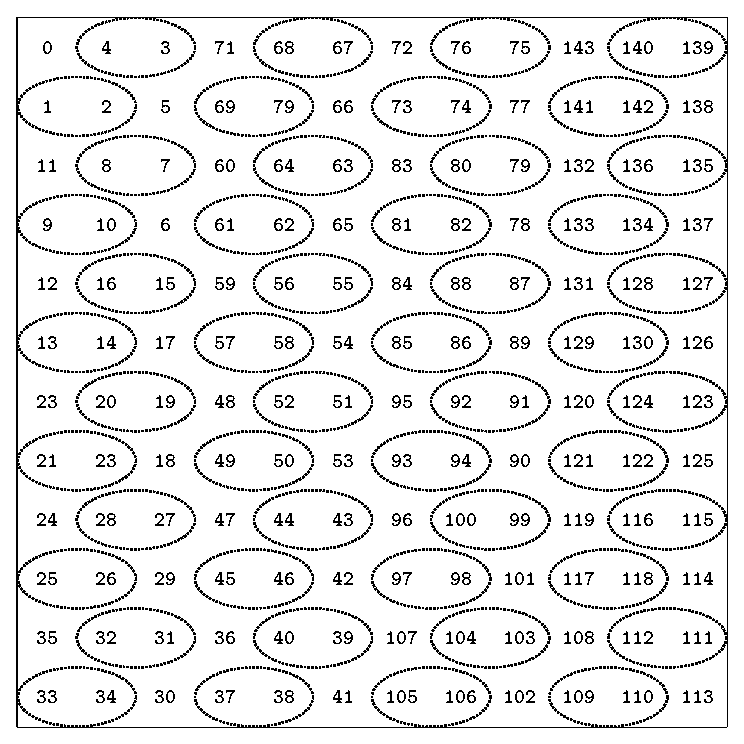
\includegraphics[scale=0.45]{order}
\caption{\small {\tt FFMA}s instruction scheduling to compute a $12\times 12$ block of C.  The numbers in
cells denote the {\tt FFMA} execution order. Dashed ellipses across two adjacent cells mean that two adjacent {\tt FFMA} instructions are dual issued in one clock cycle.}
\label{fig:order}
\end{center}
\end{figure}

\begin{figure}[htbp]
\begin{center}
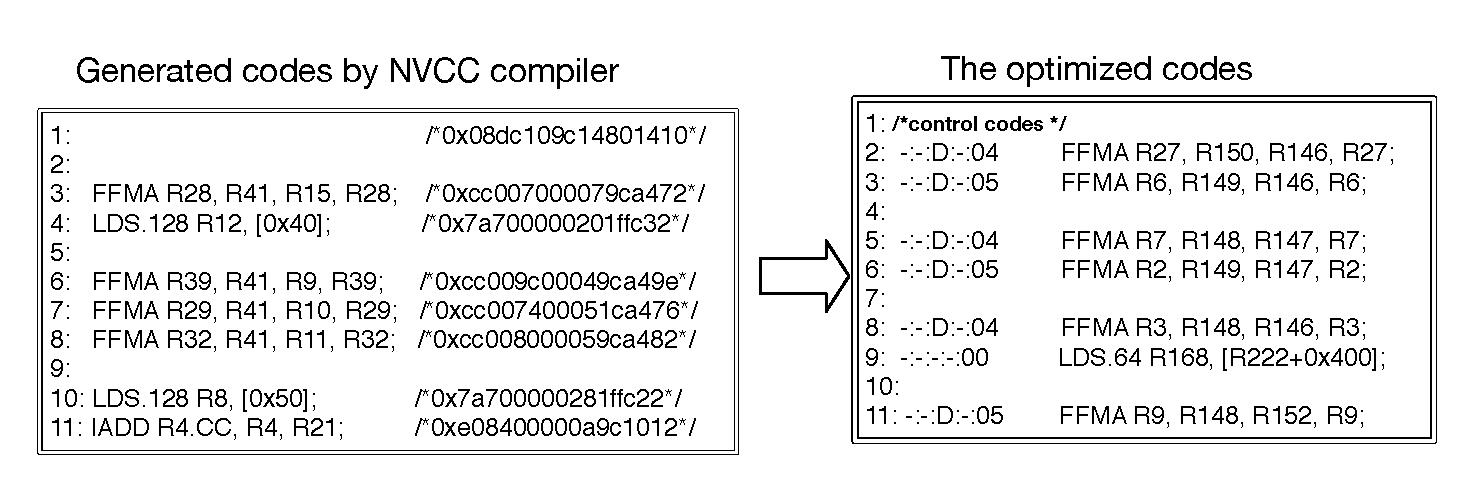
\includegraphics[scale=0.35]{assemlycode}
    \caption{\small The comparison of compiler generated codes and our tuned assembly codes.}
\label{fig:assemblycode}
\end{center}
\end{figure}
\subsection{FFMA Dual Issue}
\label{sec:ffma-dual}

It is unrealistic to keep warp schedulers dual issue the same kinds of arithmetic instructions (i.e., {\tt FFMA}) all
the time. Because on Kepler architecture, each warp is assigned $32$ cores privately, four warp schedulers will consume
$128$ cores. The reminding $192-128=64$ cores are divided into two 32-core groups, each $32$ cores
are shared by two warp schedulers. Two warp schedulers must negotiate who will use the extra $32$ shared cores to avoid
resource conflict.
As noted in {\em observation 3}, the best pattern of {\tt FFMA} instructions block is a sequence of one single issue(1
{\tt FFMA}), two dual issues (4 {\tt FFMA}s), and one single issue ((1 {\tt FFMA})). As shown in
Figure~\ref{fig:assemblycode}, the instructions in lines 3-4 and lines 6-7 are dual issued separately.
The other two instructions in line 8 and line 11 are two single issues in terms of floating-point instruction
execution.
As a comparison, most of the {\tt FFMA}s are single issued in the CUDA compiler generated codes.

By extending the basic $7$-instruction block (section~\ref{sec:benchmark}), we depict the scheduling pattern of computing a $12\times 12$ sub-block of matrix C in Figure~\ref{fig:order}.
% illustrates the order of $144$ {\tt FFMA}s instruction execution for calculating a $12\times 12$ subblock of matrix C.
For example, the {\tt FFMA} to calculate $C_{00}$ is issued first.
Then, two {\tt FFMA}s to
compute $C_{10}$ and $C_{11}$ are simultaneously issued. %We arrange all the {\tt FFMA} instructions of SGEMM according to the order in Figure~\ref{fig:order}.

Another advantage of this execution order is less register pressure due to register reuse, which can facilitate the
operand collector mechanism~\cite{collector}. The operand collector allows operand to be cached and reused in the subsequent instructions.
%is a storage element coupled with register file and
%provides inputs to the data path of the processor core for executing an instruction. %\jled{This is not the first occurrence of Operand collector.}
The assembly code in Figure~\ref{fig:assemblycode} lists the instructions to calculate $C_{32},C_{22}, C_{21}, C_{30},
C_{31}, C_{20}$, corresponding to the orders of $6,7,8,9,10,11$ in Figure~\ref{fig:reg}.
With the elaborately designed computing order and register allocation, the reuse happens as follows. The {\tt FFMA} in
Line $3$ uses cached operand {\tt R150} of line $2$, while Line $3$ and Line $4$ share {\tt R146}. Thus, in dual issue mode,
{\tt FFMA} of Line $3$ and $4$ need to read four registers {\tt R146}, {\tt R27}, {\tt R149}, {\tt R6} instead of six
registers. The corresponding banks of these registers are $0,1,3,2$ based on Table~\ref{tab:reg}, so no bank conflicts happen.
Similarly, Line 7 uses the cached operand {\tt R149} from the Line 4. In dual issue mode, two {\tt FFMAs} of Line 6 and
Line 7 need to read $4$ registers {\tt R148}, {\tt R147}, {\tt R7} and {\tt R2}.

\subsection{Schedule non-FFMA Instructions}
After setting the order of {\tt FFMA}s, {\tt non-FFMA} instructions need to be inserted in proper positions to
assure the correctness without losing performance. To tolerate instruction latency, the
distance of dependent instructions needs to be larger than their latency. The distance is approximated as
{\small
\begin{equation}
\label{eq:inst}
distance = \frac{4\times\#instructions}{7}.
\end{equation}
}
A $7$-instruction scheduling block costs four clock cycles \jli{delete: to be issued} in the dual-issue mode.
Therefore, given the distance $L$ of two interleave instructions, at least $\frac{L*7}{4}$ instructions are needed.
% two instructions of $L$ distance, then $\frac{L*7}{4}$ instructions are needed.
Besides, the number of the rest slots to insert these \jli{{\tt non-FFMA}} instructions is estimated as

{\small
\begin{displaymath}
\#slots = \frac{r_x\times r_y\times b_k}{ffmas\_in\_schedule\_block}=\frac{12\times 12\times 4}{6}=24\times 4.
\end{displaymath}
}
$r_x\times r_y\times b_k$ yields the total number of {\tt FFMA}s for one thread inside the register blocking loop \jli{inner for loop} in Algorithm~\ref{gemm}, where $r_x$ and $r_y$ are register blocking sizes and $b_k$ is the unrolling factor.
$ffmas\_in\_schedule\_block$ is the number of {\tt FFMA} instructions of one scheduling block, which is six by our
$1$-$2$-$2$-$1$ dual-issue pattern in Section~\ref{sec:benchmark}.
According to these principles, we first arrange {\tt LDS}, {\tt STS}, {\tt LDG} because of their long latencies. The
schedule slots are illustrated in two dimensions in Table~\ref{tab:position}.
Note that we use double buffers to hide the {\tt LDG} latency from global memory, which is $120$ clock cycles.
Every four loops require two {\tt LDG}s to load data from global memory to registers, four {\tt STS}s to store data from
registers to shared memory. A read after write (RAW) dependency exists between {\tt
LDG} and {\tt STS}.
From Equation~\ref{eq:inst}, $\frac{120\times 7}{4} = 210$ instructions are needed between them.
We put {\tt LDG} and  {\tt STS} in position $P[77][3]$ and $P[65][2]$ respectively in Table~\ref{tab:position}.
Thus, the in-between $143-77 + 144\times 2 + 65=419$ ($>210$) instructions are enough to hide the latency of {\tt LDG}s.
% resulting in a distance of $\frac{4\times 419}{7}=239$ clocks,.

The arrangement of {\tt LDS}s, loading data from shared memory for double buffering $A$ and $B$, follows the same approach with {\tt LDG}s.
The {\tt LDS} latency is $28$ clock cycles, thus $\frac{28\times 7}{4}=49$ instructions are needed to interleave a {\tt LDS} and a {\tt FFMA}.
In Table~\ref{tab:position}, {\tt LDS} in $P[11][3]$ reads data from {\tt STS} in $P[65][2]$,
the distance between them is more than $28$ cycles.
At the end, a {\tt BAR.SYNC} is inserted after {\tt STS} but before {\tt LDS} to make sure that data in shared memory is ready.
Other instructions such as {\tt XOR}, {\tt IADD}, and {\tt ISETP} are inserted according to data dependency; they do not influence the performance because of their short latencies.
\begin{table}[htbp]
\caption{\small The position table of {\tt non-FFMA} instructions. The inner-loop is unrolled by four times. The first column
records slot numbers and the first row represents iteration numbers.}
\label{tab:position}
\captionsetup{font=scriptsize}
\center
\scalebox{0.60} {
\begin{tabular}{|c|c|c|c|c|}
\hline
\diagbox[width=4em, height=3em]{slot}{unroll} & 0 &1 &2 &3 \\
    \hline
    5 & ISET P0 & IADD A0 & & XOR smB \\
    \hline
    11 & LDS.64 smA & LDS.64 smA & LDS.64 smA & LDS.64 smA \\
    \hline
    17 & LDS.64 smA & LDS.64 smA & LDS.64 smA & LDS.64 smA \\
    \hline
    23 & LDS.64 smA & LDS.64 smA & LDS.64 smA & LDS.64 smA \\
    \hline
    29 & LDS.64 smA & LDS.64 smA & LDS.64 smA & LDS.64 smA \\
    \hline
    35& IADD K, -4 & IADD A1 & TEXDEPBAR & \\
    \hline
    41 & LDS.64 smB & LDS.64 smB & LDS.64 smB & LDS.64 smB \\
    \hline
    47 & LDS.64 smB & LDS.64 smB & LDS.64 smB & LDS.64 smB \\
    \hline
    53 & LDS.64 smB & LDS.64 smB & LDS.64 smB & LDS.64 smB \\
    \hline
    59 & LDS.64 smB & LDS.64 smB & LDS.64 smB & LDS.64 smB \\
    \hline
    65 & & &STS.64 writeS & ISETP P2 \\
    \hline
    71 & & & & \\
    \hline
    77 & & IADD B0 & & LDG A \\
    \hline
    83 & LDS.64 smA & LDS.64 smA & LDS.64 smA & LDS.64 smA \\
    \hline
    89 &ISETP P3 & & &\\
    \hline
    95 & LDS.64 smA & LDS.64 smA & LDS.64 smA & LDS.64 smA \\
    \hline
    101 & & & STS.64 loadB0 & LDG B \\
    \hline
    107 & & & STS.64 loadB2 & XOR writeS \\
    \hline
    113 & & & & \\
    \hline
    119 & LDS.64 smB & LDS.64 smB & LDS.64 smB & LDS.64 smB \\
    \hline
    125 & & & XOR smA & \\
    \hline
    131 & LDS.64 smB & LDS.64 smB & LDS.64 smB & LDS.64 smB \\
    \hline
    137 & & & & \\
    \hline
    143 & & IADD B1 & BAR.SYNC & BAR Loop \\
    \hline
\end{tabular}
}
\end{table}

\subsection{Memory Movement}
% According to the optimization observation on memory access suggested by microbenchmark,
According to our benchmarking observations, we use {\tt LDG.128} to load data from global memory through texture cache
and {\tt LDS.64} to load data from shared memory.
Additional reasons to adopt them in SGEMM kernel are:
First, {\tt LDG.128} reduces load instructions, hence reduces {\tt non-FFMA}s. %\jled{use load instead of non-FFMA. Use non-FFMA seems complicated.}
In the inner loop of Algorithm~\ref{gemm}, we need three {\tt LDG.128}s instead of twelve {\tt LDG.32}s to read twelve
words from a $A$ column. Second, the shared memory transaction size of a warp is at most
$256$ bytes, which forces {\tt LDS.128} memory requests being split into
multiple transactions.
As we analyzed in Section~\ref{sec:experiment}, {\tt LDS.128} has a lower bandwidth than {\tt LDS.64}, which bounds SGEMM performance.

